\documentclass{article}
\usepackage[utf8]{inputenc}

\title{Advanced Programming Labwork 3}
\author{Tom HERBRETEAU }
\date{October 2018}

\usepackage{natbib}
\usepackage{graphicx}
\usepackage{pgfplots}
\pgfplotsset{compat=newest}

\begin{document}

\maketitle
Every performance measures are done on ICT4 with eiffel.jpg, without counting the image saving.
\section{Introduction}
We used CUDA instructions to make the labwork 1 faster. The RGB to gray conversion last around 65ms ! (instead of undreads before)
The gray image is also not glitched. (Remember the clouds of the first gray image with omp).
\section{Result}
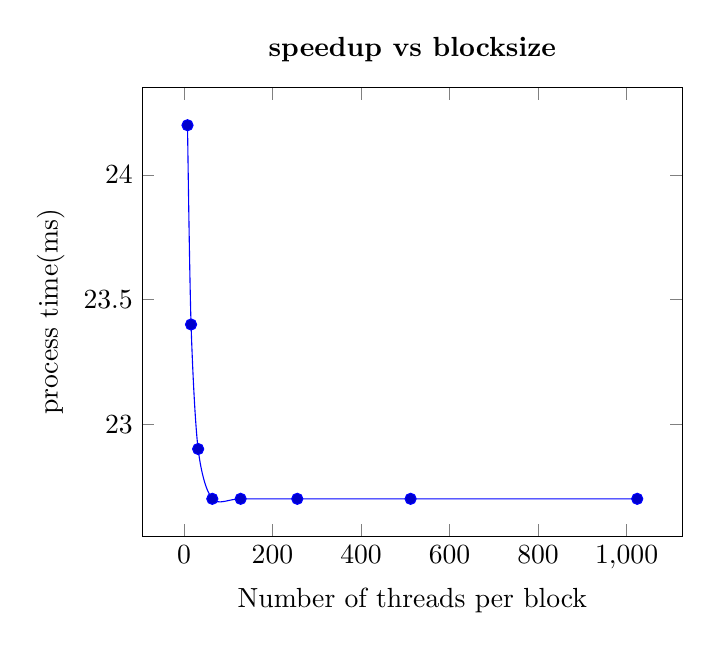
\begin{tikzpicture}
    \begin{axis}[title={\textbf{speedup vs blocksize}}, xlabel={Number of threads per     block}, ylabel={process time(ms)}]
        \addplot+[smooth,mark=*] plot coordinates
            {(8, 24.2) (16, 23.4) (32, 22.9) (64,22.7) (128, 22.7) (256,22.7) (512,22.7) (1024, 22.7)};
    \end{axis}
\end{tikzpicture}
\newline
With this parameter, we can not observe any speedup after 32 threads per block. Maybe with a bigger image or with a more complex kernel, blocksize can increase or decrease speed up. For the next labs, to be sure we don't go over the maximum number of block, we gonna work with 1024 threads per block.
\newline
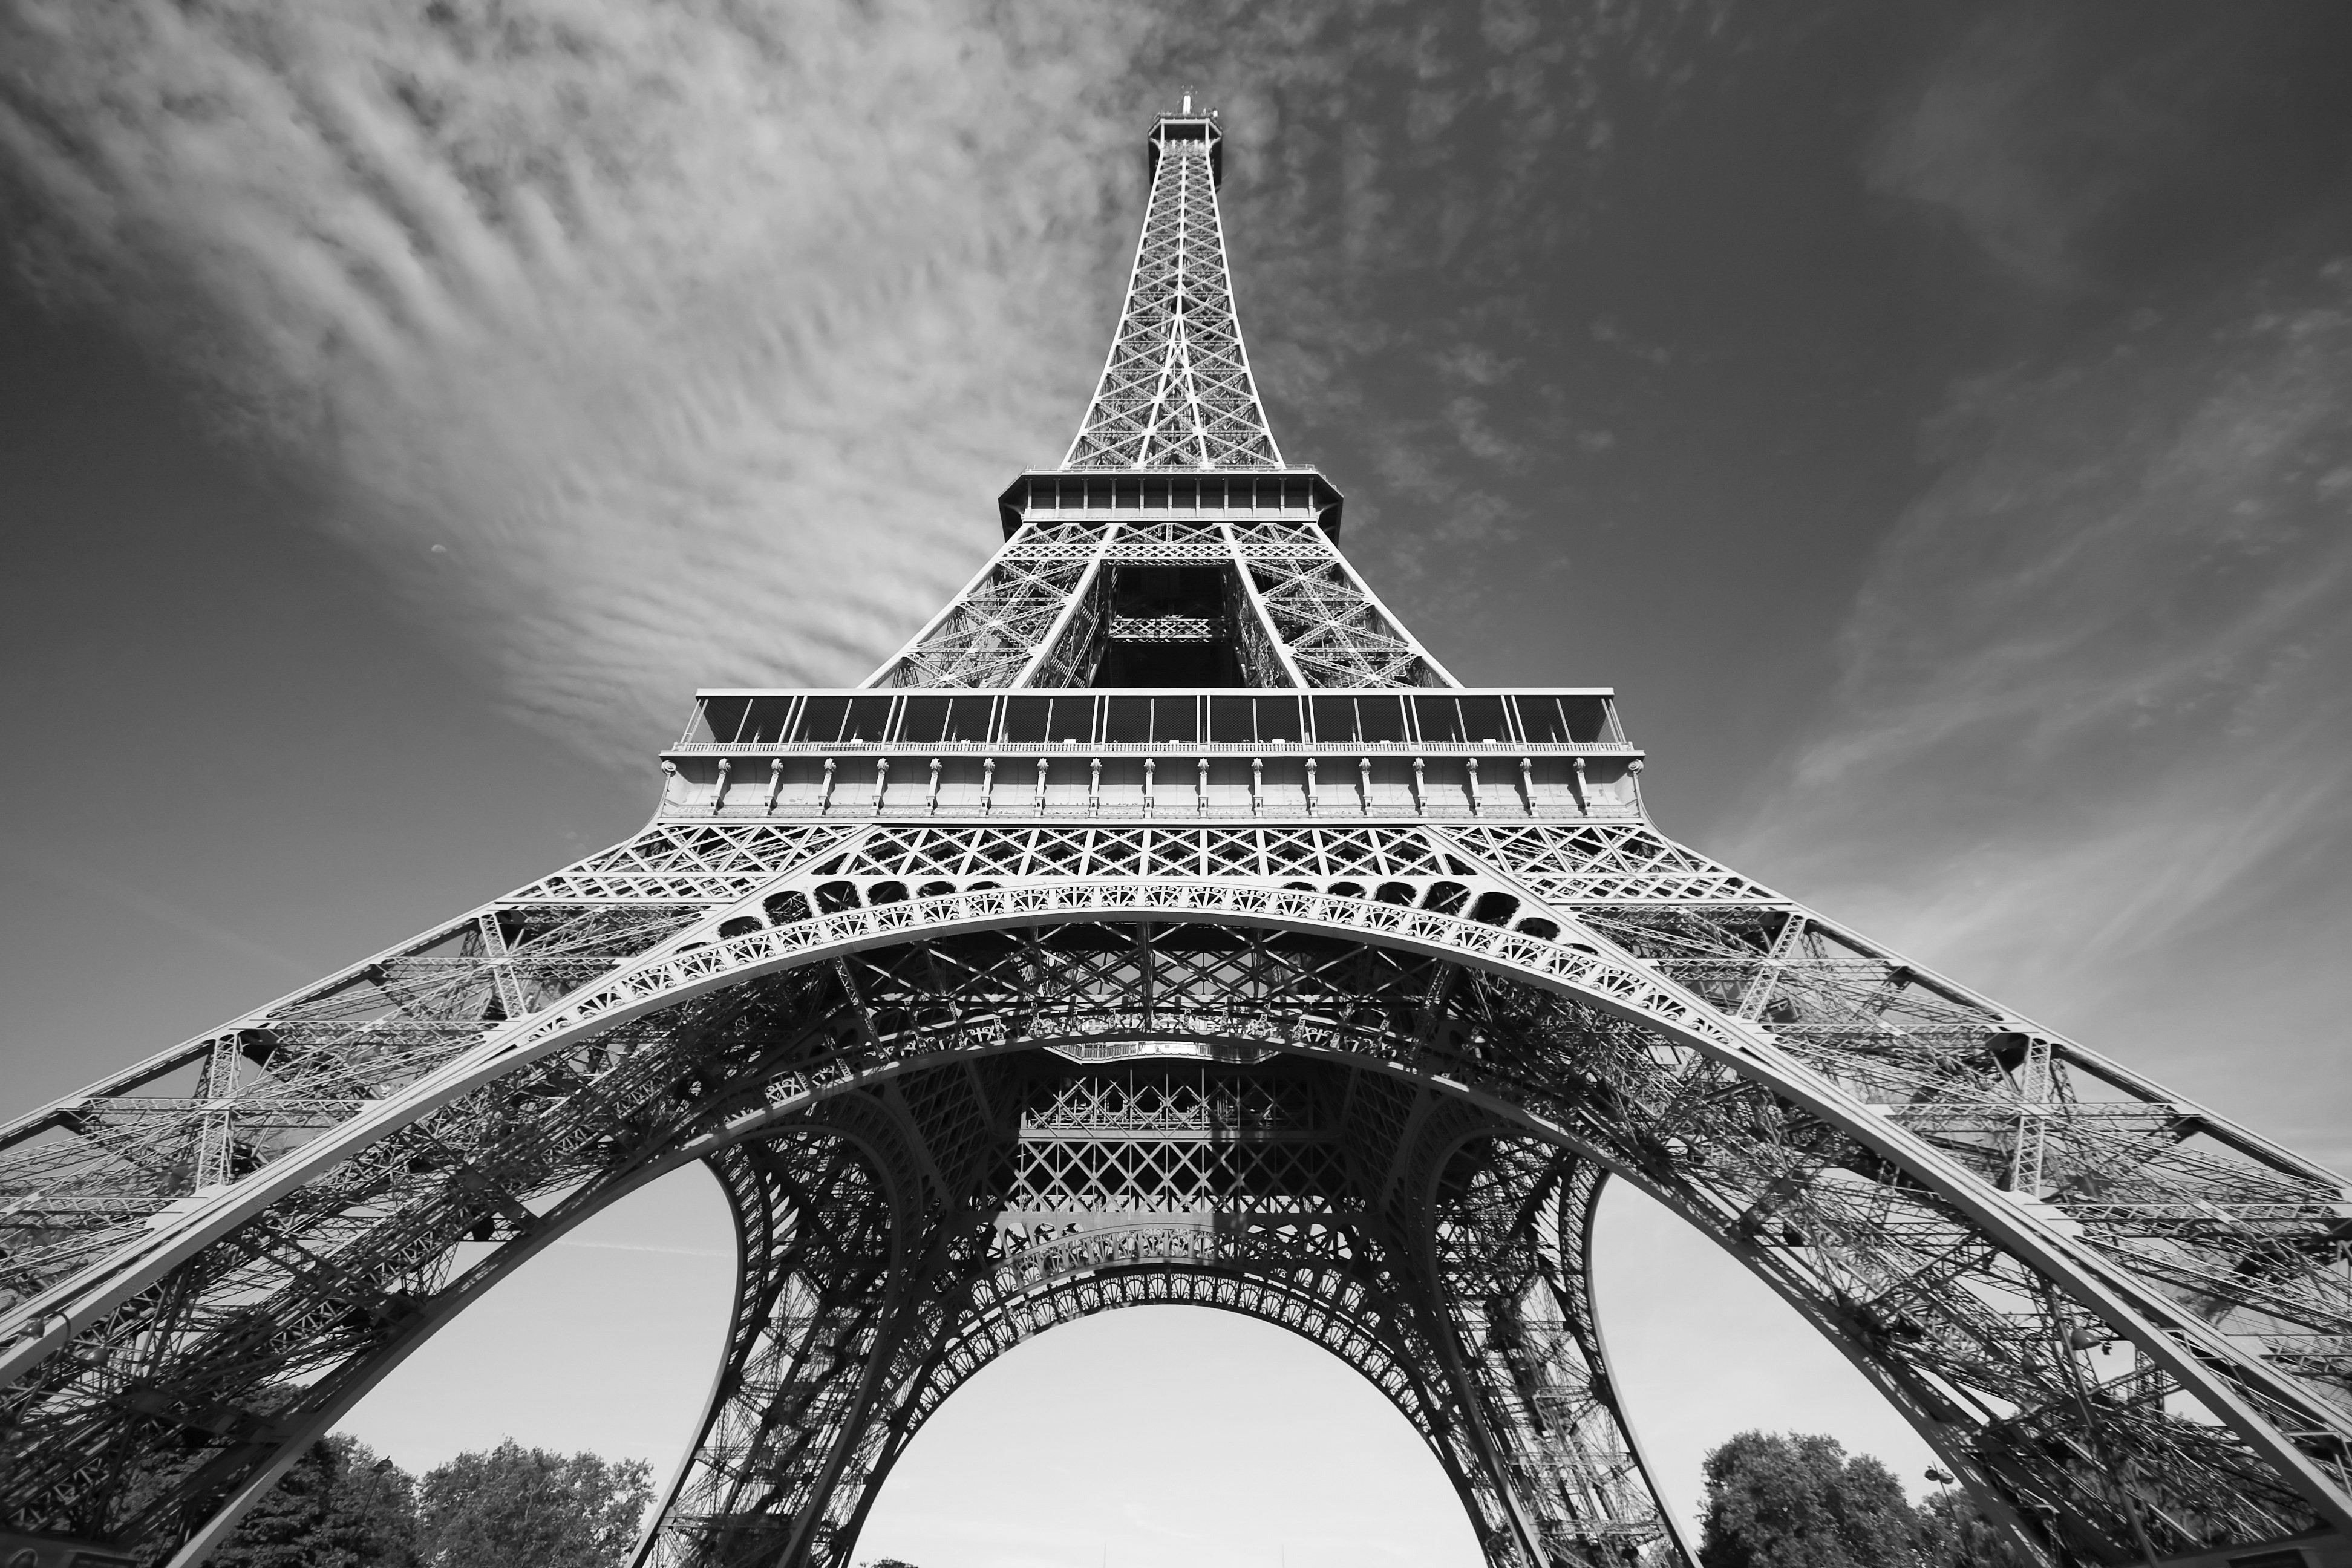
\includegraphics[width=\textwidth]{labwork3-gpu-out.jpg}
\bibliographystyle{plain}
\end{document}
